\documentclass[a4paper]{article}

\usepackage{color}
\usepackage{url}
\usepackage[utf8]{inputenc} % make weird characters work
\usepackage{graphicx}
\usepackage[margin=2.7cm]{geometry}
\usepackage[english,serbian]{babel}
\usepackage{blindtext}
\usepackage[most]{tcolorbox}
\usepackage{float}
\usepackage{amsthm}
\usepackage{tablefootnote}
\usepackage{contour}
\usepackage[unicode]{hyperref}
\hypersetup{colorlinks,citecolor=green,filecolor=green,linkcolor=blue,urlcolor=blue}
\renewcommand{\footnotesize}{\fontsize{10}{12}\selectfont}
\theoremstyle{definition}
\newtheorem{primer}{Primer}[section]
\newtheorem{teorema}{Teorema}
%\renewcommand{\lstlistingsname}{Kôd}

\usepackage{listings}
\definecolor{mygreen}{rgb}{0,0.6,0}
\definecolor{mygray}{rgb}{0.9,0.9,0.9}
\definecolor{mymauve}{rgb}{0.58,0,0.82}
\definecolor{myblue}{rgb}{0.9, 1, 0.98}


\begin{document}

\title{Optimalno uparivanje u proizvoljnom grafu\\ \textbf{- The blossom algorithm -}\\ \small{Seminarski rad u okviru kursa\\Konstrukcija i analiza algoritama 2,\\ Matematički fakultet}}

\author{\textbf{\textit{Nevena Mijailović}}, 1067/2023,\\\textbf{\textit{Marija Bogavac}}, 1068/2023,\\ \small{nevena.mijailovic000@gmail.com},\\\small{marijabogavac001@gmail.com}}
\maketitle

\abstract{
U domenu teorije grafova, koncept optimalnog uparivanja igra ključnu ulogu u različitim događajima u stvarnom svetu, kao što je uparivanje ljudi za ples na žurci, uparivanje mentora sa studentima ili usklađivanje zadataka sa radnicima u distribuiranim sistemima.

Esej počinje razjašnjavanjem teorijske osnove uparivanja u grafovima, zatim se uvodi Blossom algoritam i njegovo poređenje sa algoritmima namenjenim rešavanju istog problema. Štaviše, razmatraju se računarski aspekti Blossom algoritma, uključujući njegovu vremensku složenost i praktična razmatranja implementacije.

%Štaviše, esej istražuje praktične primene optimalnog uparivanja i Blossom algoritma u različitim domenima, uključujući optimizaciju protoka mreže, alokaciju resursa u računarskim mrežama i probleme stabilnog braka. Primeri iz stvarnog sveta ilustruju kako su efikasnost i efektivnost algoritma doprineli rešavanju složenih problema uparivanja u različitim kontekstima.

Konačno, esej se završava naglašavanjem značaja optimalnog uparivanja u teoriji grafova i nezamenljive uloge koju igra Blossom algoritam u efikasnom rešavanju takvih problema. Naglašava se svestranost i primenljivost algoritma, naglašavajući njegovu trajnu relevantnost u savremenim računarskim i algoritamskim metodologijama.
 }

\tableofcontents

\newpage

\section{Problem optimalnog uparivanja}
Za zadati neusmereni graf G=(V,E) uparivanje je skup grana koje nemaju zajedničke čvorove.\\ \textbf{Optimalno uparivanje} je uparivanje sa maksimalnim brojem grana.\cite{knjiga1}\\ Maksimalno uparivanje je pak uparivanje koje se ne može proširiti dodavanjem nove grane.\\ Svako optimalno uparivanje je maksimalno, ali nije svako maksimalno uparivanje optimalno \ref{fig:slika 1}.
\begin{figure}[H]
\begin{center}
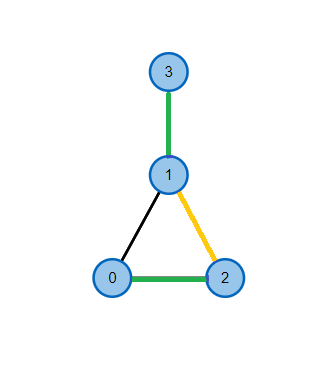
\includegraphics[scale=0.7]{graf1.png}
\end{center}
\caption{Primer maksimalnog (žuta boja) i optimalnog uparivanja (zelena boja) u grafu}
\label{fig:slika 1}
\end{figure}
\textbf{Bipartitni graf} je graf čiji se čvorovi mogu podeliti na dva disjunktna podskupa
tako da u grafu postoje samo grane između čvorova iz različitih podskupova.
Neka je G = (V, E, U) bipartitni graf u kome su V i U disjunktni skupovi čvorova,
a E je skup grana koje povezuju neke čvorove iz V sa nekim čvorovima iz U. \\

Edmondsov Blossom algoritam izračunava optimalno uparivanje u opštem grafu. Za razliku od mnogih drugih algoritama, graf ne mora biti bipartitan. On proširuje ideju Hopkroft-Karp algoritma, koji izračunava optimalno uparivanje za bipartitni graf, tako što tretira neparne cikluse na odgovarajući način.
\section{Rešenje problema optimalnog uparivanja za bipartitne grafove}	
Ukratko rekapituliramo osnovne koncepte Hopkroft-Karp algoritma koji su takođe relevantni za Edmondsov Blossom algoritam.\\ Da bismo poboljšali dato uparivanje, pokušavamo da pronađemo alternirajući put.\\ \textbf{ Alternirajući put} je putanja koja počinje slobodnim (neuparenim) čvorom, završava se neuparenim čvorom i naizmenično se smenjuju grane koje nisu i jesu u uparivanju. \\Ako smo pronašli alternirajući put, možemo poboljšati trenutno uparivanje tako što ćemo invertovati grane duž putanje: one koje nisu bile u uparivanju, sada će biti u uparivanju, a one koje jesu, neće biti u uparivanju. Time povećavamo kardinalnost uparivanja za 1. \\ \\
Na slikama \ref{graf 2 maksimalan} i \ref{graf 2 optimalan} prikazan je primer pronalaska alternirajućeg puta polazeći od maksimalnog uparivanja. Čvorovi 2 i 5 su neupareni i možemo pronaći alternirajući put između njih. Dobili smo novo uparivanje koje ima jednu granu više od prethodnog uparivanja.
\begin{figure}[H]
\begin{center}
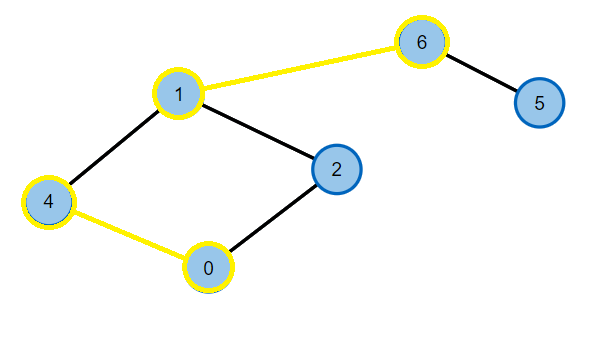
\includegraphics[scale=0.7]{Graf 2 - maksimalan.png}
\end{center}
\caption{Maksimalno uparivanje u grafu}
\label{graf 2 maksimalan}
\end{figure}

\begin{figure}[H]
\begin{center}
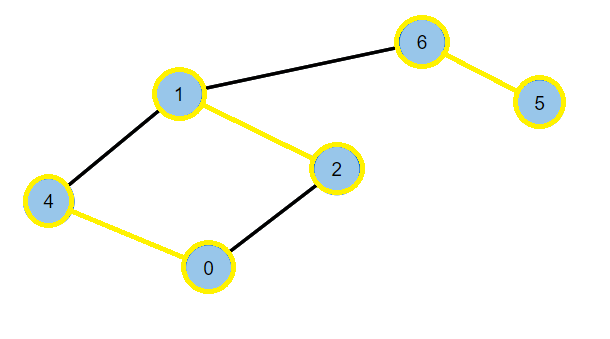
\includegraphics[scale=0.7]{Graf 2 - optimalan.png}
\end{center}
\caption{Optimalno uparivanje dobijeno pronalaskom alternativnog puta i invertovanjem grana}
\label{graf 2 optimalan}
\end{figure}


\begin{teorema}
\textsl{(O alternirajućem putu) Uparivanje je optimalno ako i samo ako u odnosu na njega ne postoji alternirajući put.}
\end{teorema}
 Prema tome, ako više ne možemo da pronađemo alternirajući put u grafu, uparivanje mora biti maksimalno.\\ \\
\textbf{Kako možemo pronaći alternirajuće putanje u grafu?} \\ \\ Prvo biramo proizvoljan slobodni čvor r i odatle pokrećemo modifikovanu pretragu u širinu (BFS). Dok prelazimo preko grafa, konstruišemo slojevito stablo sa korenom r. Grane od parnih do neparnih slojeva su neuparene grane, grane od neparnih prema parnim slojevima su uparene.\\
 Složenost ovog algoritma je $O(|V|(|V|+|E|))$ - za BFS je potreban $O(|V|+|E|)$ i ovaj proces će možda morati da se ponovi $|V|$ puta da bi alternirajuća putanja bila pronađena.\\ Postoji i poboljšanje ovog algoritma, tako što se traži više alternirajućih puteva odjednom, ali za njih mora važiti da su disjunktni putevi. Tada je složenost $O(\sqrt{V}(|V|+|E|))$.\\

Za bipartitne grafove važi da nemaju cikluse neparne dužine. \textbf{Kako onda naći optimalno uparivanje u grafovima koji sadrže i neparne cikluse?}
\newpage
\section{Opis Blossom algoritma}
Ideja blossom algoritma je da se ciklus neparne dužine u grafu može kontrakovati (skupiti) u jedan čvor tako da se pretraga za alternirajućim putevima može nastaviti iterativno kroz sada smanjeni graf\cite{sajt2} (slika \ref{fig:slika 44}). Ovde se ciklus neparne dužine naziva cvet (\textbf{blossom}). Stabljika (\textbf{stem}) je put od neuparenog čvora do cveta, a vrh (\textbf{tip}) je čvor koji spaja stabljiku i cvet. Poslednja grana stabljike do cveta (ta grana sadrži vrh) je uvek uparena. Zaista, ako bi poslednja grana stabljike bila neuparena, to bi značilo da bi se alternirajući put mogao dalje produžiti dodavanjem još jedne neuparene grane, tako da opet dobijamo da je grana koja povezuje stem i blossom uparena.\\ U cvetu postoji $2k+1$ grana od kojih tačno $k$ pripada uparivanju.\cite{sajt1} Ovo znači da postoji tačno jedan specijalni čvor u ciklusu koji nije uparen ni sa jednim drugim čvorom u ciklusu. \\ \\

Algoritam počinje od neuparenog čvora, prolazi se kroz grane do drugih neuparenih čvorova i grane se dodaju u uparivanju. Kada se dođe do maksimalnog uparivanja, tada se traže alternirajući putevi koji bi uparivanje povećali do optimalnog. Svaki put kada dodamo neuparenu granu, proverićemo da li je detektovan ciklus neparne dužine tj. blossom. Ako jeste, skupimo taj blossom u jedan čvor i tražimo alternirajući put u tako smanjenom grafu do drugog neuparenog čvora. Kada nađemo tu putanju i povećamo uparivanje, otvaramo blossom i pravilno rekonstruišemo alternirajući put kroz cvet.\\ Algoritam se zaustavlja kada nema više alternirajućih puteva u grafu to jest kada uparivanje postane optimalno.
\\
\\
\textbf{Vremenska složenost algoritma}\\ \\
Na početku postoji $|V|$ slobodnih čvorova. Za svaki od tih čvorova izvršavamo pretragu u širinu da bismo pronašli alternirajući put, koja radi u vremenskoj složenosti $O(|V|+|E|) = O(|E|)$ za povezane grafove. Pored BFS-a, moramo izvršiti najviše $|V|$ kontrakcija (a samim tim i najviše $|V|$ proširenja). Jedna kontrakcija (proširenje) se može izvršiti u vremenu $O(|E|)$ jer u najgorem slučaju moramo da skupimo sve čvorove i grane u jedan čvor. Nakon što smo pronašli alternirajući put, invertovanje grana u najgorem slučaju zahteva vreme $O(|V|)$. Sve u svemu, ovo dovodi do ukupnog vremena rada $O(|V| \cdot (|E|+|E||V|+|V|))=O(|V|^2|E|)$.
\\ \\
\textbf{Kako se algoritam može poboljšati?} \\ \\
Postoji mnogo prostora za poboljšanje performansi algoritma. Neke ideje Mikalijevog i Vaziranijevog algoritma dodatno smanjuju vreme rada na $O(\sqrt{|V|}|E|)$:
\begin{itemize}
\item Umesto da izvodimo BFS iz jednog slobodnog čvora, mogli bismo da pokrenemo BFS iz svih slobodnih čvorova istovremeno. Na taj način možemo pronaći nekoliko disjunktnih alternirajućih puteva odjednom i povećati kardinalnost uparivanja za više od 1.
\item Ne moraju se svi cvetovi odmah skupiti. Postoji takozvani uslov cvetanja koji određuje da li moramo da sklopimo ciklus neparne dužine ili možemo to da odložimo.
\item Posebna tehnika obeležavanja omogućava brzo širenje cvetova.
\end{itemize}
Štaviše, Edmonds tvrdi da, pod određenim okolnostima, "superčvorovi" (čvorovi nastali skupljanjem cvetova) mogu biti ostavljeni kontrahovani sve dok njihovo proširenje nije zaista potrebno \cite{knjiga2}. U našoj implementaciji, proširujemo sve superčvorove u grafu kada pronađemo putanju za povećanje, ali u mnogim slučajevima to nije neophodno.

\newpage
\begin{figure}[H]
\begin{center}
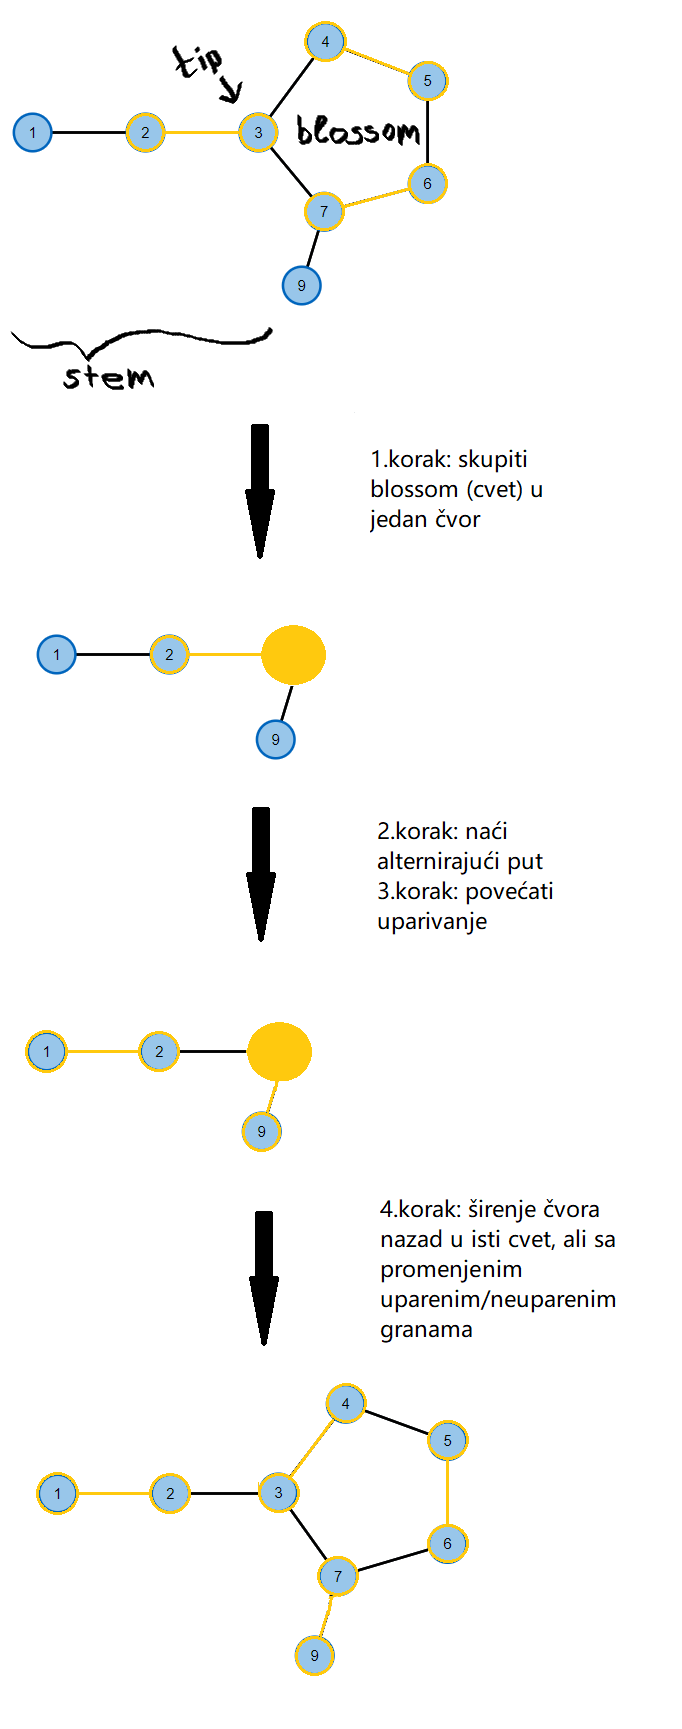
\includegraphics[scale=0.63]{Screenshot (363).png}
\end{center}
\caption{Primer upotrebe blossom algoritma na proizvoljnom grafu}
\label{fig:slika 44}
\end{figure}

\section{Implementacija Blossom algoritma}

\section{Primeri i vizualizacija Blossom algoritma}

\section{Poređenje sa drugim algoritmima}
Uporedićemo blossom algoritam sa Hopkroft-Karp algoritmom i Ford-Fulkersonovim algoritmom.

\begin{table}[ht]
\centering
\begin{tabular}{|l|c|p{4cm}|p{1.8cm}|p{4cm}|}
\hline
\textbf{Algoritam} & \textbf{Tip grafa} & \textbf{Ključna ideja} & \textbf{Vremenska složenost} & \textbf{Karakteristike}\\
\hline\hline
\textbf{\textit{Blossom}} & Opšti & Koristi tehnike skupljanja za iterativno smanjenje ciklusa neparne dužine (cvetanja) dok se podudaranje ne može proširiti & $O(n^{3})$ & Dokazano je da je optimalan u najgorem slučaju za pronalaženje optimalnog uparivanja u opštim grafovima \\
\hline
\textbf{\textit{Hopkroft-Karp}} & Bipartitni & U jednoj pretrazi se pronalazi veći broj
alternirajućih puteva koji moraju biti međusobno nezavisni (disjunktni) & $O(n^{2.5})$ & Brz za bipartitne grafove, ali nije primenljiv na opšte grafove (koji mogu da sadrže neparne cikluse) \\
\hline
\textbf{\textit{Ford-Fulkerson}} & Opšti & Oslanja se na tehnike maksimizovanja protoka u transportnoj mreži & $O(n^{5})$ & Nije tako efikasan u praksi zbog proizvoljnog izbora povećavajućeg puta \tablefootnote{U opštem slučaju, kada su kapaciteti grana celobrojni vreme izvršavanja Ford-Fulkersonovog algoritma može biti $O(|E| \cdot f)$, gde je sa f označen maksimalni tok kroz mrežu. Edmonds i Karp su 1972. godine pokazali
da ako se među mogućim povećavajućim putevima u rezidualnom grafu uvek
bira onaj sa najmanjim brojem grana, onda je broj povećavanja najviše $(|V||E|)$,
te je ukupna složenost algoritma $O(|V||E|)$}. \\

\hline

\end{tabular}
\end{table}

\begin{tcolorbox}[width=393pt,colback={myblue},title={Ključna razmatranja za izbor algoritma},colbacktitle=mygray,coltitle=black,boxrule=0.5pt,boxsep=3pt]  
\begin{itemize}  
\item Tip grafa: Bipartitni ili opšti?
\item Vremenska efikasnost: Koliko je brzina ključna za rad aplikacije? 
\item Složenost implementacije: Da li su detalji implementacije algoritma zadovoljavajući?
\item Opšte preporuke:\\
- Za opšte grafove: Blossom algoritam je često poželjan izbor zbog njegove efikasnosti i sposobnosti da rukuje bilo kojom strukturom grafa.\\
- Za bipartitne grafove: Hopkroft-Karp algoritam je generalno brži i jednostavniji za implementaciju.
\end{itemize}
\end{tcolorbox} 
\newpage
\section{O autoru Blossom algoritma}
Džek Edmonds rođen je 1934. godine u SAD-u. On je doktor računarskih nauka i dobitnik Džon fon Nojmanove nagrade za izuzetne doprinose.
\begin{figure}[ht]
\begin{center}
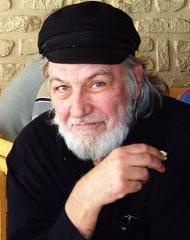
\includegraphics[scale=0.4]{jack_edmonds.jpg}
\end{center}
\caption{Džek Edmonds}
\label{fig:slika 6}
\end{figure}
\\Ključne oblasti gde se ističe uticaj Edmondsa:
\begin{itemize}
\item Kombinatorna Optimizacija: Edmonds se smatra jednim od osnivača ove oblasti, koja se fokusira na pronalaženje "najboljeg" rešenja među velikim brojem mogućnosti. Njegov Blossom algoritam za optimalna uparivanja u grafovima, razvijen 1961. godine, ostaje temelj ove oblasti.

\item Poliedarska Kombinatorika: Dao je značajan doprinos razvoju poliedarskih metoda, koristeći geometrijske oblike za predstavljanje i rešavanje problema optimizacije.

\item  Teorija Računarske Složenosti: Ova oblast istražuje inherentnu težinu računarskih problema. Edmondsov rad, posebno njegov članak iz 1965. godine "Paths, Trees and Flowers," pripisuje se za iniciranje razvoja matematičke teorije efikasnih kombinatornih algoritama.
\end{itemize}

\section{Zaključak}
Ovde su navedene neki primeri iz stvarnog sveta koji ilustruju kako su efektivnost algoritma doprineli rešavanju složenih problema uparivanja u različitim kontekstima.
\begin{itemize}
\item \textit{Optimizacija mrežnog toka}\\
     U optimizaciji mrežnog toka, Blossom algoritam se može koristiti za pronalaženje maksimalnog protoka ili minimalnog preseka u mreži. Određivanjem optimalnog protoka resursa kroz mrežu, obezbeđuje se efikasno korišćenje resursa i optimalne performanse mrežnih sistema kao što su transportne mreže, telekomunikacione mreže i mreže lanca snabdevanja.

\item \textit{Alokacija resursa u računarskim mrežama}\\ Računarske mreže se često suočavaju sa izazovima u vezi sa alokacijom resursa, gde resursi kao što su propusni opseg, procesorska snaga ili skladištenje moraju biti optimalno dodeljeni različitim korisnicima ili zadacima. Blossom algoritam može pomoći u maksimalnom korišćenju resursa dok zadovoljava ograničenja, čime se povećava efikasnost i performanse računarskih mreža.

\item \textit{Problemi sa stabilnim brakom}\\ U kontekstu stabilnih bračnih problema, gde svaki skup muškaraca i žena ima preferencije za potencijalne partnere, Blossom algoritam se može koristiti za pronalaženje stabilnih uparivanja koje zadovoljavaju određene kriterijume, kao što je osiguranje da nijedan par pojedinaca ne bi više voleo jedni druge u odnosu na trenutne partnere. Ova aplikacija ima praktične koristi u platformama za pronalaženje provodadžija, dodeljivanju poslova i drugim scenarijima gde preferencije treba uzeti u obzir.
\end{itemize}
Ovi primeri pokazuju svestranost Blossom algoritma u rešavanju različitih problema optimizacije i uparivanja u različitim domenima, pokazujući njegovu praktičnu važnost u efikasnom rešavanju izazova u stvarnom svetu. 


\newpage

\addcontentsline{toc}{section}{Literatura}
\appendix
\bibliography{seminarski} 
\bibliographystyle{plain}

\appendix


\end{document}
